\documentclass[
	english,%globale Übergabe der Hauptsprache
%	logofile=example-image-duck, %Falls die Logo Dateien nicht vorliegen
	authorontitle=true,
	]{bfhbeamer}


\usepackage[main=english]{babel}
\usepackage{tikz}  
\usepackage{tikzsymbols}
\usepackage{tikzducks}
\usepackage{amsmath}
\usepackage{caption}

% Der folgende Block ist nur bei pdfTeX auf Versionen vor April 2018 notwendig
\usepackage{iftex}
\ifPDFTeX
\usepackage[utf8]{inputenc}%kompatibilität mit TeX Versionen vor April 2018
\fi


%Makros für Formatierungen der Doku
%Im Allgemeinen nicht notwendig!
\let\code\texttt

\title{Bachelor Thesis}
\subtitle{Extended BBS Signature}
\author[J. Robles]{Joel Robles}
\institute{TI}
\titlegraphic*{\includegraphics{example-image-duck}}%is only used with BFH-graphic and BFH-fullgraphic

%Activate the output of a frame number:
%\setbeamertemplate{page number in head/foot}[framenumber]


\AtBeginSection{\sectionpage}

\begin{document}

\maketitle

\begin{frame}{Table of Contents}
    \tableofcontents
\end{frame}

\begin{frame}{Preface}
    \framesubtitle{Buying a Swisspass}
    \begin{columns}[onlytextwidth,T]
        \column{50mm}  
        
        \centering
        \textbf{Client}\newline\newline
        
\begin{tikzpicture}
            \duck[graduate]
        \end{tikzpicture}

        \column{50mm}

        $$\underrightarrow{\includegraphics[width=30mm]{example-image-duck}}$$
        $$\overleftarrow{\includegraphics[width=30mm]{example-image-duck}}$$

        \column{50mm}

        \centering
        \textbf{SSB}\newline\newline
        \centering
        
\begin{tikzpicture}
            \duck[tshirt, jacket=blue!50!black, tie=red]
        \end{tikzpicture}

    \end{columns}
\end{frame}

\begin{frame}{Preface}
    \framesubtitle{Signing a phone contract}
    \begin{columns}[onlytextwidth,T]
        \column{50mm}  
        
        \centering
        \textbf{Client}\newline\newline
        
\begin{tikzpicture}
            \duck[graduate]
        \end{tikzpicture}

        \column{50mm}

        $$\underrightarrow{\includegraphics[width=30mm]{example-image-duck}}$$
        $$\overleftarrow{\includegraphics[width=30mm]{example-image-duck}}$$

        \column{50mm}

        \centering
        \textbf{Swiss Post}\newline\newline
        \centering
        
\begin{tikzpicture}
            \duck[tshirt, jacket=yellow!50!orange, tie=black]
        \end{tikzpicture}

    \end{columns}
\end{frame}

\begin{frame}{Preface}
    \framesubtitle{Colluding verifiers}
    \begin{columns}[onlytextwidth,T]
        \column{50mm}  
        
        \centering
        \textbf{SSB}\newline\newline
        \centering
        
\begin{tikzpicture}
            \duck[tshirt, jacket=blue!50!black, tie=red]
        \end{tikzpicture}

        \column{50mm}

        $$\underrightarrow{\includegraphics[width=30mm]{example-image-duck}}$$
        $$\overleftarrow{\includegraphics[width=30mm]{example-image-duck}}$$

        \column{50mm}

        \centering
        \textbf{Swiss Post}\newline\newline
        \centering
        
\begin{tikzpicture}
            \duck[tshirt, jacket=yellow!50!orange, tie=black]
        \end{tikzpicture}

    \end{columns}
\end{frame}

\section{Tasks}

\begin{frame}{Tasks}
    \begin{itemize}
        \item VCs \& OIDC4VP
        \item Pseudonyms
        \item Link Secrets \& Blind Signatures
    \end{itemize}
\end{frame}

\section{VC's \& OIDC4VP}

\begin{frame}{VC's}
    \begin{figure}[h]
        \centering
        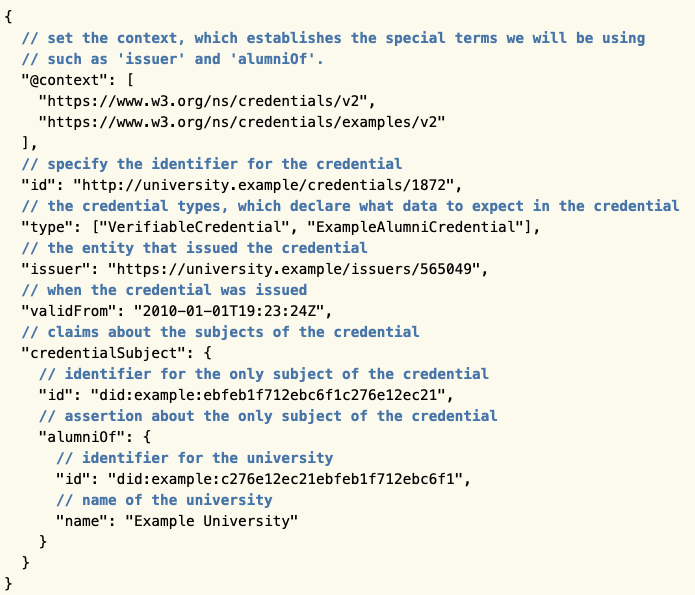
\includegraphics[width=70mm]{./img/VC_example.png}
        \caption{Example of a VC, \url{https://www.w3.org/TR/vc-data-model-2.0/}}
    \end{figure}
\end{frame}

\begin{frame}{Problems with VC's}
    \begin{itemize}
        \item No Java implementation for VC's
        \item ID in the VC as well as in the credentialSubject (making VC's linkable)
        \begin{itemize}
            \item The ID in the credentialSubject can be left out. If we want to have revocation the Credential needs to have an ID.
        \end{itemize}
        \item How do we sign the attributes of the credentialSubject but also the whole credential for data Integrity, in a way that we can leverage the selective disclosed of BBS?
        \begin{itemize}
            \item Flatten the JSON Object
        \end{itemize}
    \end{itemize}
\end{frame}

\begin{frame}{OIDC4VP}
    \begin{figure}[h]
        \centering
        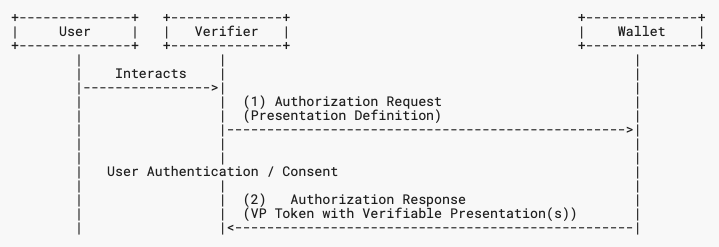
\includegraphics[width=120mm]{./img/OIDC4VP.png}
        \caption{Same Device Flow for OIDC4VP, \url{https://openid.net/specs/openid-4-verifiable-presentations-1_0.html}}
    \end{figure}
\end{frame}

\section{Pseudonyms}

\section{Link Secrets \& Blind Signatures}


\end{document}

